\question
(Fall 2016) Draw the environment diagram for the following code.

\begin{minipage}{\textwidth}
\begin{lstlisting}
lamb = 'da'
def da(da):
    def lamb(lamb):
        nonlocal da
        def da(nk):
            da = nk + ['da']
            da.append(nk[0:2])
            return nk.pop()
    da(lamb)
    return da([[1], 2]) + 3

da(lambda da: da(lamb))
\end{lstlisting}
\end{minipage}

\begin{solution}[0.5in]
\begin{center}
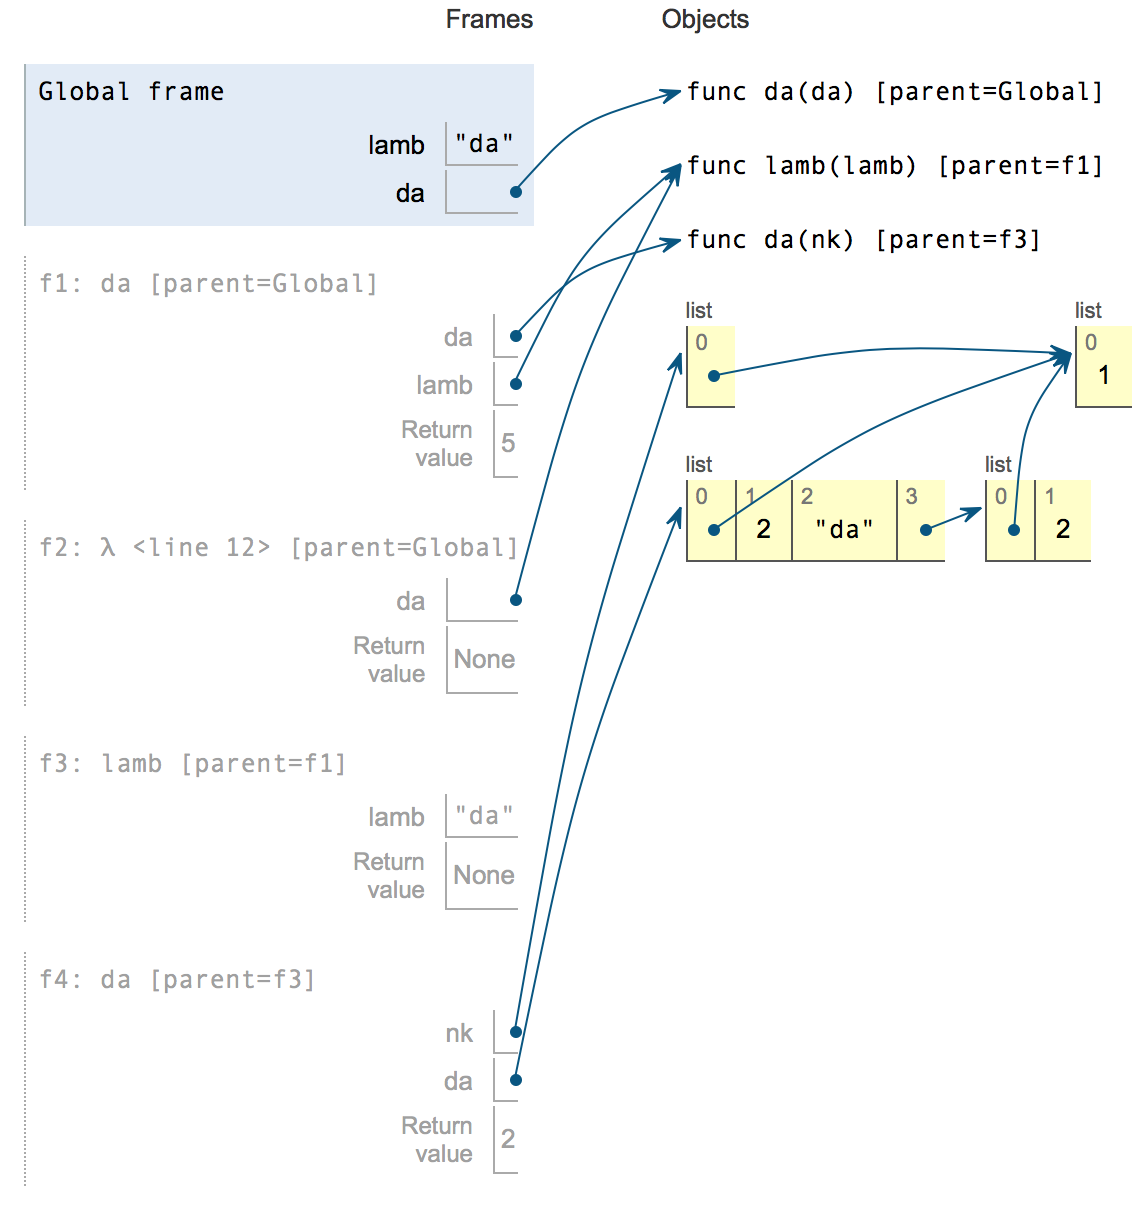
\includegraphics[scale=.5]{dalamb.png}
\end{center}
\end{solution}
